
\documentclass[fleqn,12pt]{article}

\usepackage[margin=15mm]{geometry}
\usepackage[utf8]{inputenc}
\usepackage[bulgarian]{babel}
\usepackage[unicode]{hyperref}
\usepackage{amsfonts}
\usepackage{amssymb}
\usepackage{enumitem, hyperref}
\usepackage{upgreek}
\usepackage{indentfirst}
\usepackage{graphicx}

\usepackage{amsmath}

\graphicspath{ {./img/} }

\title{Тема 16 \\Модели и методи за проектиране на потребителски интерфейс.}

\author{v0.1}
\date{26 юни 2021}

\begin{document}

\maketitle
\tableofcontents
\pagebreak

\section{Основни  модели  и  методи  при  създаване  на  потребителски  интерфейс}

\textbf{\textit{Дейността по проектиране на човеко-машинен интерфейс}} включва \textbf{проектиране, създаване и оценяване} на интерактивни компютърни системи, предназначени за използване от хора.
\bigbreak
Основно значение има взаимодействието между един или повече потребители с една или повече програми, които те използват. 

% lection 9
\subsection{Подходи}

Основните подходи са:
\begin{enumerate}
    \item \textbf{Потребителя в центъра (User-centеred design (UCD))}, където потребителя е основен източник, а проектантът превежда изискванията му.
    \item \textbf{Действията в центъра (Activity-centеred design (ACD))}, който е насочен не към целите, а стъпките при всяко действие.
    \item \textbf{Системно проектиране}, където има ударение върху крайната система.
    \item \textbf{Артистично проектиране (Genius design)}, където се разчита на опита и творчеството на дизайнера, а ролята на потребителя е да потвърди дизайна.
\end{enumerate}

% lection 9
\subsection{Oсновни процеси}

Основните дейности са:
\begin{enumerate}
    \item \textit{Определяне на нуждите и установяване на изискванията}
    \item \textit{Проектиране на алтернативни решения}
    \item \textit{Избор между алтернативите(оценяване)}
    \item \textit{Създаване на прототип}
\end{enumerate}

% lection 3
\subsection{Анализ на задачите}

\textbf{\textit{Бележка}} - Явно за преподавателите по ПЧМИ думите действие и задача са едно и също нещо.

Основните методи за анализ на задачи са:
\begin{itemize}
    \item \textbf{\textit{Task Analysis}} - простите действия се разглеждат като черни кутии.
    \item \textbf{\textit{Cognitive Task Analysis}} - анализира действия, изискващи значителна умствена дейност от потребителите като решаване на проблеми, внимание и преценка.
    \item \textbf{\textit{Hierarchical Task Analysis}} - всички действия се представят като йерархия, като така по-сложните се представят като съвкупност от по-прости.
\end{itemize}

% UAN, Директно манипулируеми интерфейси -> lection 3
\subsection{Основни техники за специфициране на взаимодействията}

Взаимодействието между потребителя и интерфейса може да бъде специфицирано чрез средства като \textbf{BNF (Backus-Naur Form), граматики и диаграми}, \textbf{многозначни граматики}, \textbf{дървета от диалогови кутии}, \textbf{избор на менюта}, \textbf{диаграми за преход} и \textbf{графи на състоянията (автомати?)}.

Категориите софтуерни инструменти за спецификация на потребителските взаимодействия са:
\begin{itemize}
    \item \textit{Средства с общо предназначение} като \textbf{PowerPoint} и \textbf{Visio}.
    \item \textit{Средства за спецификация на софтуерни системи} базирани на \textbf{UML} и подобни.
    \item \textit{Специфични системи за интерфейси} като \textbf{LucidChart}.
    \item \textit{Системи за прототипиране} като \textbf{Balsamiq}.
\end{itemize}

% Powerpoint, visio or something after UAN -> lection 3
\subsection{Инструментални средства}

\textit{\textbf{User Action Notation (UAN)}} е инструмент за специфициране на потребителските действия, която \textbf{не зависи от потребителя или технологията на интерфейса}.
Тя цели да покаже \textbf{връзката между действията и интерфейсните елементи}, описвайки интерфейсите \textbf{прецизно, подробно и еднозначно}.
\bigbreak
Основна градивна единица е \textbf{действие на потребител в даден контекст}, като то се описва \textbf{сценарии} чрез \textbf{спомагателни бележки} и \textbf{диаграма на преходите между състоянията в даден сценарий при конкретни условия}. 
\bigbreak
Чрез \textbf{UAN} могат да се репрезентират \textbf{direct manipulation interfaces (DMI)}.
\textit{\textbf{DMI}} е стил на интеракция между човек и машина, при който обектите на интерфейса могат да се манипулират директно.
Например потребител да преоразмери триъгълник на екрана използвайки мишката.

% ----------------------------------------------------------
\section{Проектиране на графичен интерфейс}

% от shit архива
\subsection{Интерактивни стилове и техники}

Формите на взаимодействие на потребителя с потребителския интерфейс могат да се класифицират в 5 основни стила:
\begin{itemize}
    \item \textbf{\textit{Директно въвеждане (direct manipulation)}} - потребителят директно работи с обектите на екрана (напр. за да изтрие файл го тегли в кошчето с мишката).
    \item \textbf{\textit{Избор от меню (menu selection)}} - потребителят избира команда от списък с възможности наречен меню.
    \item \textbf{\textit{Попълване на форми (form fill-in)}} - потребителят попълва данни във форма. (като в НАП)
    \item \textbf{\textit{Команден език (command language)}} - потребителят въвежда команди и техни параметри за да укаже на системата какво да прави.
    \item \textbf{\textit{Естествен език (natural language)}} - потребитял използва естествен език. (например когато си играе със Siri или Slack chatbot-а).
\end{itemize}

% от shit архива
\subsection{Отчитане на психологичните особености на потребителите}

Отчитането на познавателните способности на потребителите има важна роля в проектирането на интерфейса.
Разграничаваме ги в две основни групи: % в shit архива са на обратно
\begin{itemize}
    \item \textbf{експериментални} -  начина ни на мислене, сравнение и вземане на решения.
    \item \textbf{рефлективни} - начина ни на действие и реакции на дадени събития.
\end{itemize}

% от shit архива
\subsection{Концептуални модели и метафори}

\textbf{\textit{Концептуалните модели}} описват системата като множество от интегрирани идеи и концепции, относно това какво трябва тя да прави, как да изглежда и какво поведение да има в конкретни ситуации.
Прилагането им спомага за ефективната употреба на потребителския интерфейс.
\bigbreak

Има няколко вида концептуални модели:
\begin{itemize}
    \item \textbf{базирани на дейностите} - описват най-основните дейности, които се извършват. (комуникация, навигация и др.)
    \item \textbf{базирани на обектите} - фокусират се върху конкретни обекти и тяхното използване в даден контекст.
    \item \textbf{смесени} - смесица от горните два.
\end{itemize}

Друг начин за описване на концептуалните модели са \textbf{\textit{метафорите}}.
Те притежават аспекти на физически обекти, но имат и свои характеристики.
По този начин те обогатяват с нови концепции знанието ни за използване на даден обект.

% Методи за създаване на интерфейси - Storyboarding, Wizard of OZ -> lection 3
\subsection{Методи и средства за реализация}

Използват се следните методи за създаване на интерфейси:
\begin{itemize}
    \item \textbf{\textit{Сценарии (Storyboarding)}} - описват как система реагира при конкретна последователност от стъпки в определена среда.
    Предимства са, че:
    \begin{itemize}
        \item \textit{се фокусират над цялата система}, т.е. как се изпълнява всяка дейност.
        \item \textit{се абстрахират от конкретика на интерфейса}.
        \item \textit{свързват се всички роли в дадена дейност за постигане на цел}.
    \end{itemize}
    \item \textbf{\textit{Хартиени прототипи}} - интерактивен хартиен прототип направен от изрезки хартия (бутончета, менюта и т.н.);
    получава се естествено взаимодействие като човек симулира работата на сървър нареждайки елементите на интерфейса.
    Предимства са, че:
    \begin{itemize}
        \item \textit{се фокусират над цялата система}
        \item \textit{скицирането е бързо, лесно и гъвкаво (вкусно)}.
        \item \textit{всички могат да участват}.
    \end{itemize}
    \item \textbf{\textit{Компютърни прототипи}} - интерактивна софтуерна симулация, където има висока прецизност на показване, но няма дълбочина (backend).
    Начин за справяне с това е да се ползва \textit{Wizard of Oz} техниката, където има скрит човек, който симулира сървъра.
    \item \textbf{\textit{Смесени прототипи}} - комбинация от горните видове.
\end{itemize}

% ----------------------------------------------------------
\section{Разработка на използваем графичен интерфейс}

\subsection{Техники базирани на експерименти}

Разработката на потребителски интерфейс включва и различни техники за оценка на постигнатото.
Провеждат се експерименти с типични потребители (лабораторни плъхове) в специално създадени лаборатории.
\bigbreak
Разпространени начини за събиране на информация за оценка са:
\begin{itemize}
    \item \textbf{\textit{Въпросници}}, които събират информация за това какво мислят потребителите за интерфейса;
    \item \textbf{\textit{Наблюдение на потребителите}} по време на работа със системата;
    \item \textbf{\textit{Кадри от видео записи}} от различно използване на системата;
    \item \textbf{\textit{Инжектиране на шпионски код}}, събиращ информация за най-използваните елементи и най-честите грешки;
    \item \textbf{\textit{Think Aloud протокол}}, където плъховете разсъждават на глас докато работят със системата.
\end{itemize}

% ----------------------------------------------------------
% reuse shit archive
\section{Разработка на мултимедиен графичен интерфейс}

Основните елементи на мултимедията са цветове, звуци, текст, графика и анимация.

\subsection{Проектиране на цветове}

Цветовете се използват с определена цел и следват модела на излъчването.
Има няколко начина за представяне на цвят, по-известните от които са:
\begin{itemize}
    \item \textbf{\textit{RGB}} - червено (red), зелено (green), синьо (blue), където интензивността на всеки цвят се задава с число $n \in [0, 255]$.
    \item \textbf{\textit{CMYK}} - циан (cyan), магента (magenta), жълто (yellow) и черно (black), където интензивността им се измерва в проценти.
    Използва се при принтерите.
    \item \textbf{\textit{HSL}} - оттенък (hue) в градуси, наситеност (saturation) в проценти и светлива (light) в проценти.
\end{itemize}

Те се използват за привличане на внимание, показ на състояние и даване на обратна връзка.
Не може без цветове.
\bigbreak

За добро съчетание на цветовете се използват цветови схеми.
Те могат да бъдат монохроматични (monochromatic), аналогични (analogous), допълващи (complementary), триъгълни (triad), правоъгълни (tetradic) и други.

\begin{center} 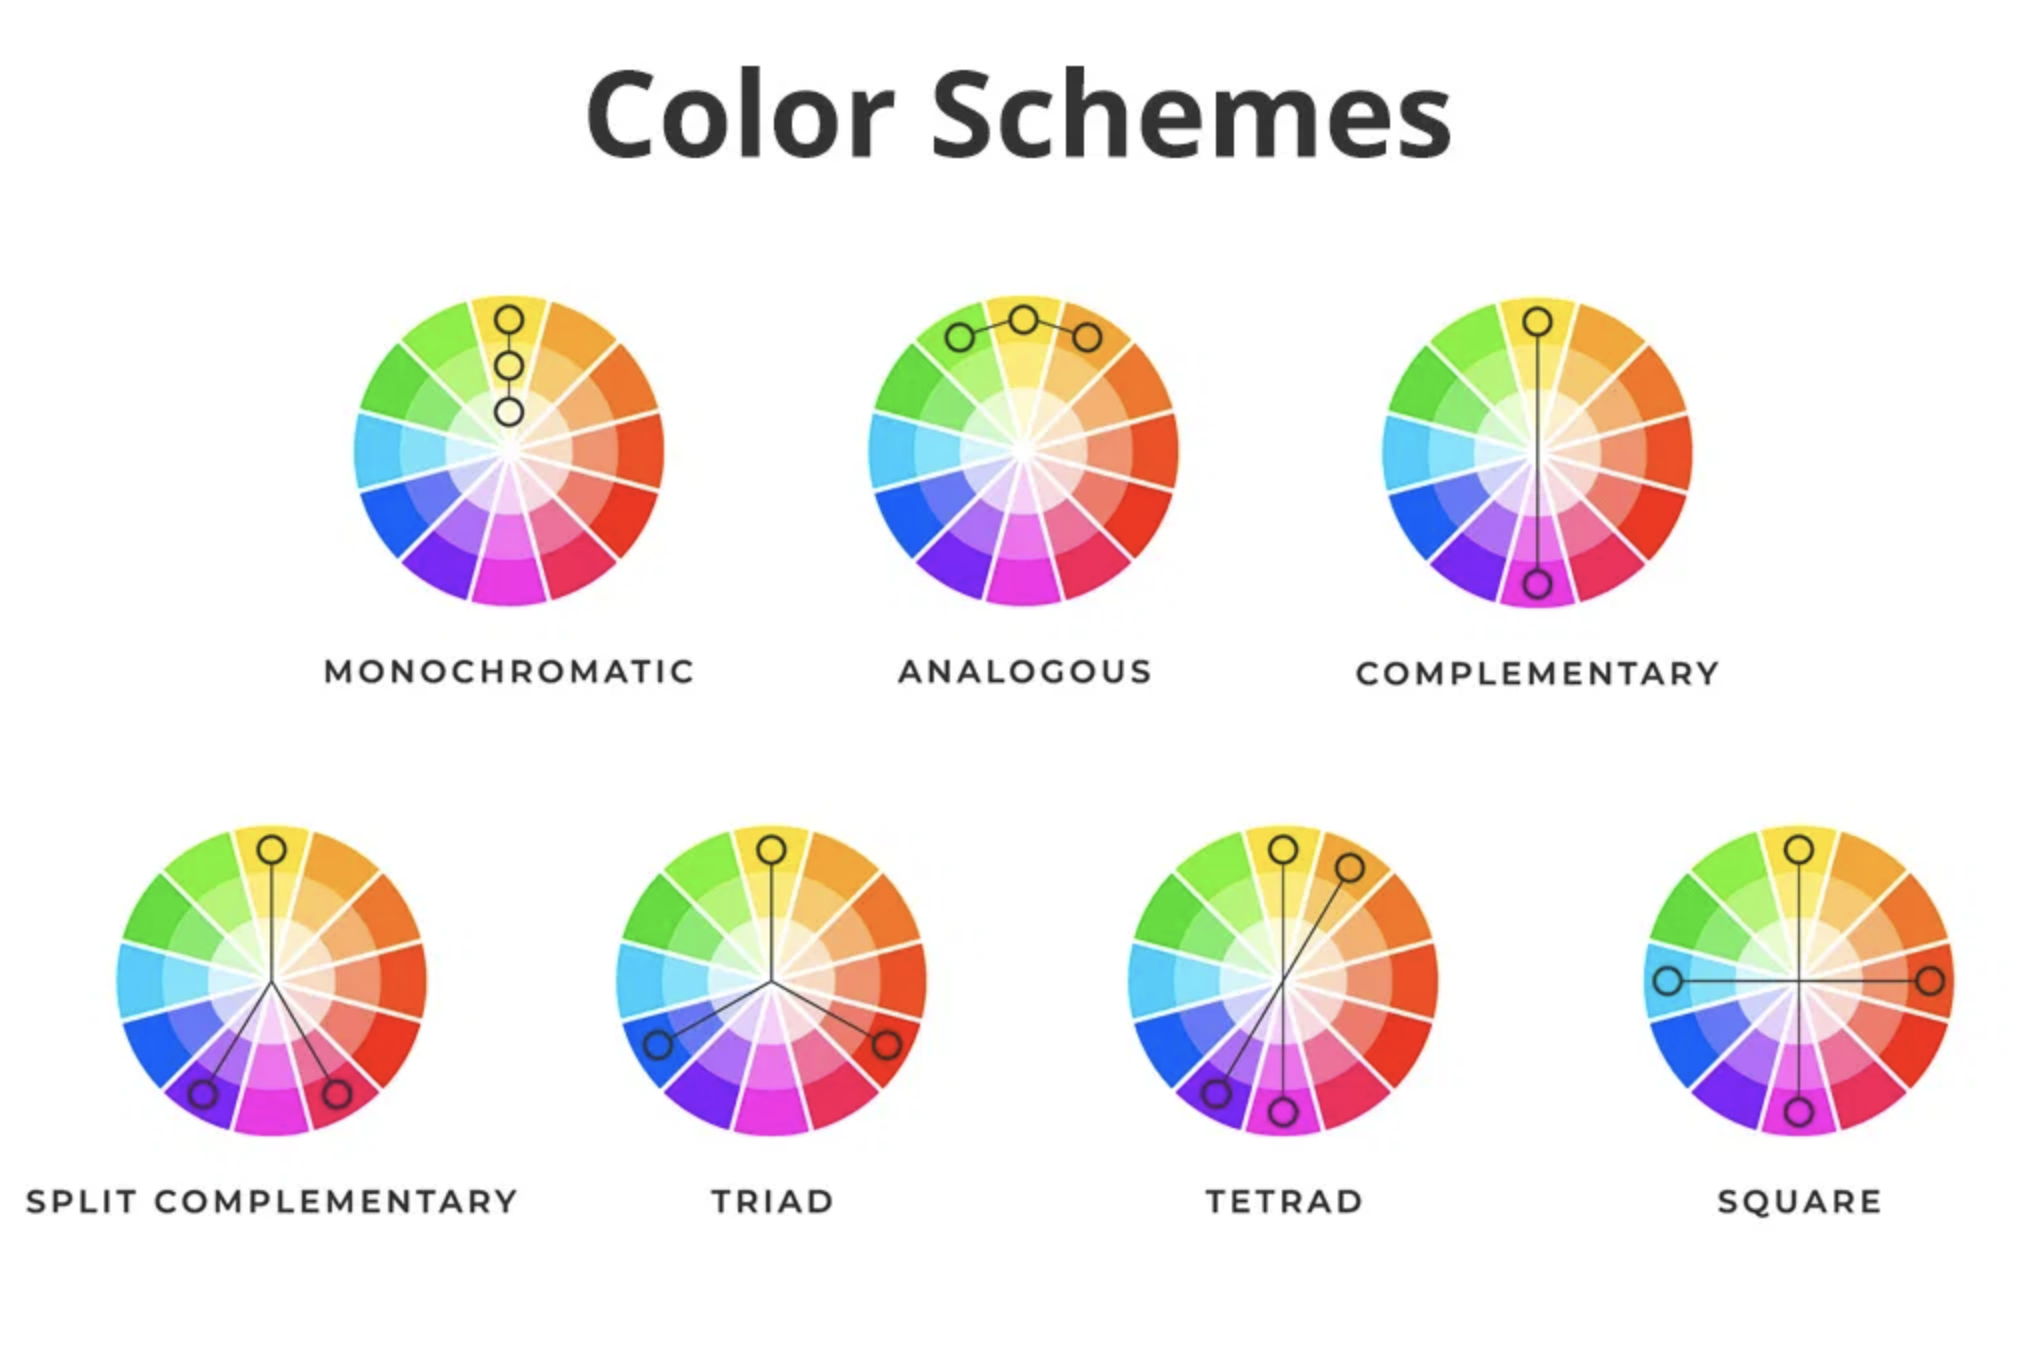
\includegraphics[width=300px]{color_schemes.png} \end{center}

\subsection{Проектиране на звуци}

Звукът се използва в 3 форми - \textbf{звуци, говор и музика}.
Интегрира се в софтуерни системи чрез формати като \textbf{mp3, wav, ogg} и други.
Той придава емоционални въздействия, обогатява с ефекти елементите на мултимедията и дава възможност на автора директно на комуникира с потребителя.

\subsection{Проектиране на текст}

Текстът е лесно преносимо средство за предоставяне на подробна информация.
Често дълъг текст е трудно четим и се налага той да бъде разбит на парчета и да се форматира.
\bigbreak

Известни текстови кодирания са:
\begin{itemize}
    \item \textbf{\textit{ASCII}} - представяне на всяка буква чрез 1 байт.
    \item \textbf{\textit{UTF-8}} - стандартно множество от символни кодирания, съдържащо много повече символи от ASCII.
    Оптимизация е, че всеки символ може да заема различен размер в зависимост от номера си.
    Например латинските букви заемат по 1 байт, а тези на кирилица по 2 байта.
\end{itemize}

\subsection{Проектиране на графика}

Графиките/Изображенията са нагледен материал, представящ визуално определена информация на малка площ. Основните начини за кодиране на изображения са:
\begin{itemize}
    \item \textbf{\textit{растерна графика}} - изображението се кодира като (двумерен) масив от цветови точки (например RGB точки).
    В последствие цветовите точки се използват за рисуване на цвят върху екрана.
    Растерните графики са добри за \textbf{представяне на детайли}, но може да има \textbf{загуба на детайли при скалиране на изображенията}.
    Известни формати са \textbf{jpg, png и gif}.
    \item \textbf{\textit{векторна графика}} - изображението се кодира като елементи представени чрез пътища зададени чрез математически формули.
    Те резултират във фигури като кръгове, триъгълници, b-сплайни и други при рисуване.
    Добре е да се използва за \textbf{симплистични обекти}, като логота и графи, защото за разлика от растерната графика не се загубват детайли при скалирането.
    Известни формати са \textbf{svg и eps}.
\end{itemize}

\subsection{Проектиране на анимация}

Анимацията представя движещи се образи, които показват състоянието на обекти под формата на графики в различни моменти от времето.
Често се използват за визуализиране на неща, които се илюстрират трудно другояче.
Известни формати за анимация са \textbf{mp4, mov и avi}.

% ----------------------------------------------------------
\section{Особености при създаване на интегриран интерфейс}

\subsection{Методи за моделиране насочени  към  крайния  потребител}

При дизайна на потребителския интерфейс основно внимание трябва да се обръща на потребителите и техните нужди.
Следователно трябва да се използват методи, ориентирани към събиране на информация от крайния потребител.
\bigbreak
Известни методи са:
\begin{itemize}
    \item \textbf{\textit{етнография}} - наблюдение на потребителите, докато извършват ежедневните си дейности;
    \item \textbf{\textit{метод на свързаността}} - комбинира етнографския подход с инженеринга на изискванията;
    \item \textbf{\textit{метод на контекстния дизайн}} - цели да улесни събирането и интерпретацията на информацията от дадена област, така че да се изпълни подходящ за нея софтуерен продукт;
    \item \textbf{\textit{метод на участието}} - за разлика от контекстния метод, потребителите участват активно в разработката, като част от екипа на дизайнерите;
\end{itemize}

\subsection{Екранен  дизайн}

При изграждане на екранния дизайн основна роля заема дизайна на иконите:
\begin{itemize}
    \item Избраната икона трябва да е \textit{ясно видима и лесно да се разграничава};
    \item Всяка икона трябва да е \textit{ясно различима};
    \item Иконите трябва да са \textit{сходни};
    \item \textit{Избягване на излишните детайли} при съставянето на иконите;
\end{itemize}

\subsection{Oбработка на взаимодействията}

Един добре изграден интерфейс трябва да поддържа обработка на взаимодействията с потребителя, като предлага:
\begin{itemize}
    \item \textit{Ясна и подробно информация}, но не повече от нужната;
    \item \textit{Еднозначни и лесни указания};
    \item \textit{Смислени и информативни съобщения за грешки};
    \item Лесен достъп до \textit{допълнителна информация и указания};
\end{itemize}

\subsection{Интерактивни методи за проектиране}

Интерактивните методи включват:
\begin{itemize}
    \item Разбиране на \textit{нивото (опит) на потребителите};
    \item \textit{Определяне на задачите} – провеждане на наблюдения и разговори;
    \item \textit{Избиране на стил на взаимодействие};
    \item \textit{Освобождаване на потребителя};
    \item \textit{Съчетаване на автоматичност и управление на потребителя};
\end{itemize}

\subsection{Прототипиране}

Прототипът представлява модел, създаден за да демонстрира новия продукт.
Целта на прототипа на интерфейса е да позволи на потребителя да добие пряк опит с използването на създадения продукт.
Това е необходимо при оценяването на интерфейса.
Процесът по прототипиране е на два етапа:
\begin{enumerate}
    \item създаване на прости (напр. хартиени) прототипи.
    \item разработване на по-сложни автоматизирани версии.
\end{enumerate}

\end{document}
